\input{./_path-to-root.ltx}
\documentclass[\PathToRoot/\ProjectName]{subfiles}
\whenstandalone{\externaldocument{\PathToRoot/\ProjectName}}

\begin{document}

\begin{figure}[H]
  \centering
  \caption{Multiplier comparison: with vs.\ without splurge factor}
  \whenintegrated{\label{fig:cumulativemultipliers_SplurgeComp}} 
  % Original path: \PathToRoot/Code/HA-Models/FromPandemicCode/Figures/Splurge0/Cumulative_multipliers_SplurgeComp
  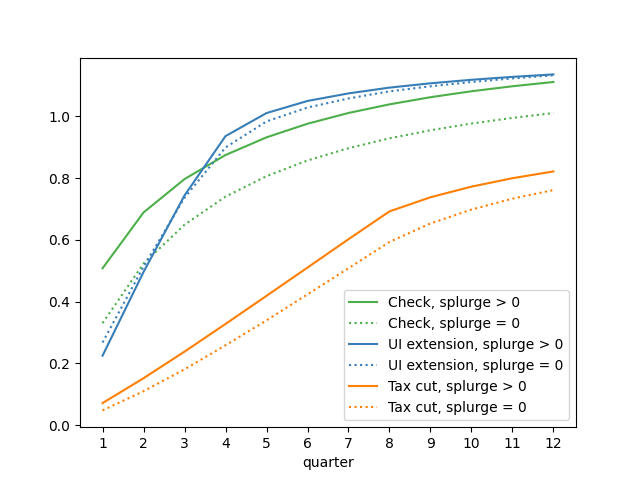
\includegraphics[width=.9\textwidth]{\PathToRoot/images/Cumulative_multipliers_SplurgeComp}
\end{figure}
\noindent\parbox{\textwidth}{\footnotesize
  \textbf{Note}: This figure compares cumulative multipliers for all three policies
  in models with and without the splurge factor (Appendix~\ref{app:Model-without-splurge}).
  Both model specifications show similar policy rankings: UI extensions remain most effective,
  followed by stimulus checks, with payroll tax cuts least effective.
  The splurge factor enhances multipliers by improving the model's ability to match
  empirical spending patterns, but does not fundamentally alter policy effectiveness rankings.
  This robustness validates the main paper's conclusions across alternative model specifications.
}

\vspace{1em}  % Add space after figure

% Smart bibliography: Only include bibliography if standalone AND has citations
\smartbib

\end{document}
